\chapter{CMOS MAPS sensors} \label{ch:CMOS}

The fourth chapter aims to introduce the essential features of the semiconductor detector technology, going through the history of its advancements, which have led to the currently most promising sensors based on CMOS logic structure, the Monolithic Active Pixel Sensors (MAPS). As we have seen in the previous chapter, the VTX program wants to make the most of the technologies that have already proven reliable in precision measurements, like the TJ-Monopix development line, with also fast readout and high radiation tolerance. We will briefly present it, mentioning the peculiarities of its prototypes, to better understand how they could fulfill the Belle II requirements.


\section{Semiconductor detectors} 

The detection of elementary particles, nuclei and radiations occurs through their interactions with matter. In particular, charged particles are often detected by atom ionization or excitation of the sensitive detector layers along the path they take passing through. This detection method can be used in gases, liquids and semiconductors. We want to focus on detectors that use semiconductors as sensitive material. \\

All solid can be divided into three categories based on their electrical conductivity: conductors, semiconductors and insulators. 
In a solid state lattice, the constituent atoms have a dense periodic arrangement and for this reason, the energy of single atoms are split due to the influence of other atoms in the vicinity. The energy levels of some level groups lie energetically so dense (order of meV) that one speaks of \emph{energy bands}, separated from each other by a \emph{band gap}, which represent the distance in energy between them (\textbf{$E_{G}$}, energy gap). The electrical conduction properties of materials are determined by the two highest energy bands, which are the \textbf{valence band (VB)} and the \textbf{conduction band (CB)}. The energy levels within the same band are so dense that the transitions to unoccupied levels, if they are not completely filled, are easly possible. Therefore the electrical conduction properties depend on the band gap between the two lavels and on the band occupation, as we can see in~\autoref{fig:energy_band}.

\begin{figure}[h!]
\centering
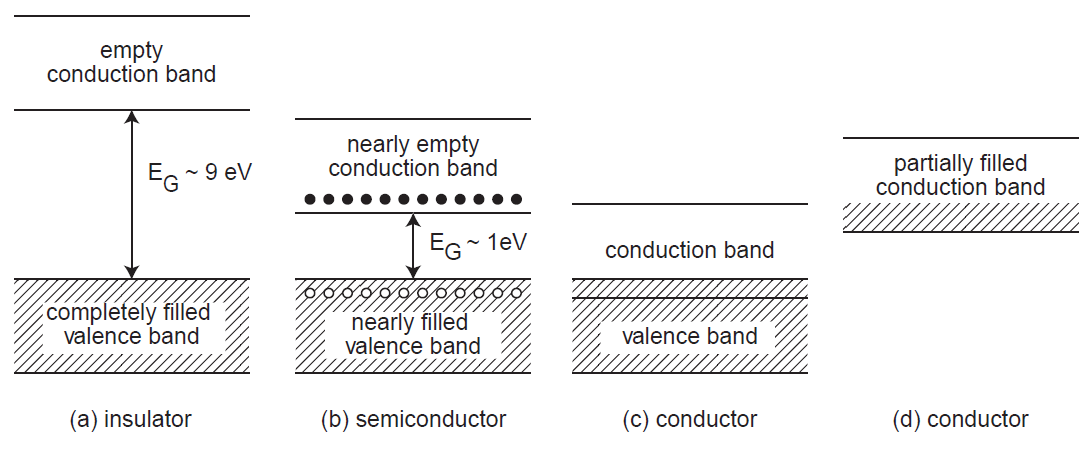
\includegraphics[scale=.6]{energy_band}
\caption{Schematic structure of the energy bands in insulators (a), semiconductors (b) and conductors (c,d).}
\label{fig:energy_band}
\end{figure}

In insulators the valence band electrons are strongly bonded to neighbouring atoms, they are not free and they do not contribute to the conduction. In fact the VB is entirely occupied, the CB instead, is empty. As a consequence of the strong interatomic bond, there are large energy gap between the VB and the CB (typically $E_{G}$ of about 9 GeV). Thus current flow is pratically impossible. 

In semiconductors weaker bonds between neighbouring atoms result in a smaller energy gap with respect to the insulator (for example 1.12 eV in silicon). In this way electrons from VB can easily overcome the gap, moving on the CB by thermal excitations or by external electric fields. When an electron makes this transition, it leaves a hole in the VB, wihch could be filled in turn by another electrons of the VB. If and electric field is applied, the free electrons in the CB and the holes in the VB start to move producing two different current flows, one negative and the other positive, respectively.

In conductors the conduction and valence band overlap or the conduction band is partially filled so transitions within the same band and between the two different bands are easy and current conductions requires minimal energy.


\subsection{Movement of charge carriers and signal formation in semiconductors}

Semiconductor materials are the only ones that allow the detection of charged particles by ionization of the sensitive matter (in conductors a current is always present, not only in case of particle or radiation crossing). 

%, mainly due to ionization, atom excitation and bremsstrahlung radiation
When a charged particle or a photon pass through the medium, they release a certain amount of energy mainly by ionization or absorbtion by semiconductor, respectively. Most part of this energy loss, in turn, causes the formation of positive and negative charges, which in this context, are defined charge carriers (the rest is absorbed by the lattice). In semiconductors these carrier are the hole electron pairs created by ionization, which  start to move in opposite direction due to an electric field: the holes (positive) migrate towards the \textit{\textbf{anode}} and the electrons (negative) towards the \textit{\textbf{catode}}, which sense the signal induced by this movement. In fact, their drift induce an accumulation of charges on the electrode surfaces, and it is possible to record this charge induction as a charge, current or voltage signal. It is worth to notice that the generation of the signal is dependent on the movement of the carriers relative to the electrodes, and not when they actually arrive, that is the moment in which the signal stop.\\

The charge carrier density of semiconductors can be modified by doping the material with specific chemical elements, and this process causes a modification of their conduction properties.
Undoped semiconductors are called \emph{intrinsic semiconductors}. \\
\emph{Extrinsic semiconductors} instead, are artificially doped with external impurities like: 

\begin{itemize}
\item Pentavalent elements (P, As, Sb), called \emph{donors}, added in a tetravalent material (Si, Ge) produce an axecss of conduction electron with respect to the holes (n doping, \autoref{fig:doping} (a)).
\item Trivalent atoms (B, Al, Ga), called \emph{acceptors}, create an excess of holes (p doping, \autoref{fig:doping} (b)).
\end{itemize}

\begin{figure}[h!]
\centering
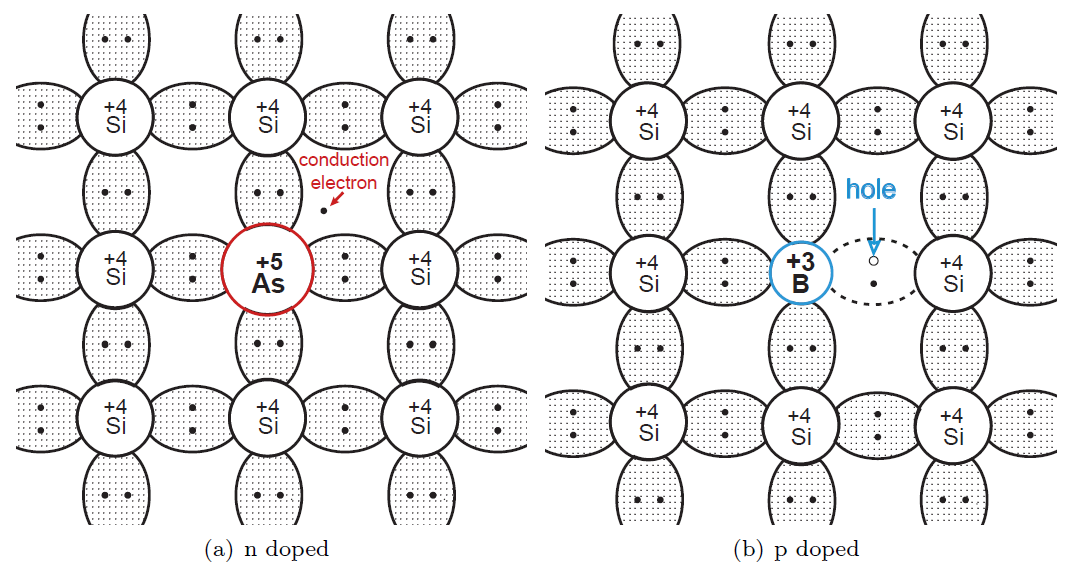
\includegraphics[scale=.5]{doping}
\caption{Schematic representation of atom bonding structure in n-doped and p-doped semiconductors.}
\label{fig:doping}
\end{figure}

%diffusion and drift?
%energy necessary to release for silicon 3.65 e numero medio elettroni prodotti??
%other semiconductor
%immagine pagina 137(signal_form), 276(pn_junction(3)), 280(depletion) KOLANOSKI
%fluttuazioni
%RAMO THEOREM
%inversion
%radiation damage

\subsection{The pn junctions as detector}

The base material employed in semiconductor detectors is silicon, which is stable, abundant and it has a low band gap which allow to produce an adequate amount of charge, enough to be detected.\\ 
When a p-doped semiconductor get in contact with a n-doped material, a \textit{pn junction} is formed. In particular, the p-doped part is the one where holes are the dominant charge carriers, called \textbf{majority carriers}; in the n-doped part of the crystal instead, the majority carriers are the electrons. 
The presence of these excesses of opposite charge in the two part of the junction, and as consequence the generation of a potential difference across the junction, causes a migration of the majority carriers from each part to the opposite one. At the boundary the charges recombine, and this process creates a zone which is free of charge carriers, called \textbf{depletion zone}. After the recombination the atoms of this depletion region are ionized and so it is no longer neutral, but features a \emph{space-charge}: a positive one in the n-layer, and a negative in the p-layer. Moreover these space charge densities are opposite in sign, so they generate an intrinsic electrical field that stop the original diffusion.\\

%RECOMBINATION
[NOTE ON RECOMBINATION]

Moreover, the application of an external voltage $V_{ext}$ between the two section of the junction, provokes a variation of the width of the depletion region, depending on the size and polarity of the applied voltage. It is possible to distinguish:

\begin{itemize}
\item \emph{forward bias}, $V_{ext}$>0: a positive external voltage applied to the p side with respect to the n side, causes a reduction of the depletion region ???
\item \emph{reverse bias}, $V_{ext}$<0: if a negative voltage at the p side or positive at the n side relative to the respectively opposite side is applied, the depletion region gets wider.
\end{itemize}

Depleted region is a zone without free charge carriers (do not come from the signal), and with the presence of an external eletric field (reverse bias), this is a fundamentals for semiconductor detectors.

The performance of the junction as a detector is determined above all by the boundary properties between p-and n- doped silicon. Boundaries of the same doping type, but with different concentration, also create a similar pn structure, like for example $n^{+}n$ or $p^{+}p$. There are also Metal-semiconductor boundaries, used in metal contact with the outside and Metal-Oxide-Semiconductor interfaces (MOS) that we will see in more details in the following.
 
 
\subsection{Complementary Metal-Oxide-Semiconductor (CMOS)}

A MOS structure is a double interface make of three different media: an insulator (oxide) placed between the metal and the semiconductor, as shown in~\autoref{fig:mos}.

\begin{figure}[h!]
\centering
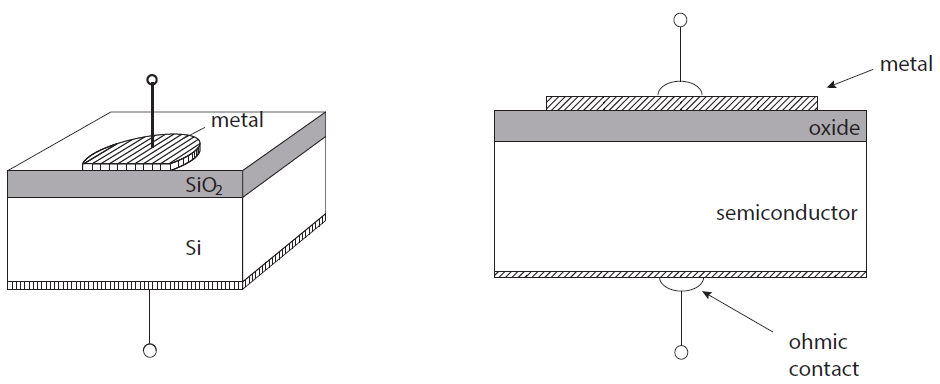
\includegraphics[scale=.6]{mos}
\caption{A perspective (on the left) and a cross-sectional illustration (on the right) of a MOS structure.}
\label{fig:mos}
\end{figure}

In recent transistor technology, the metal is almost entirely replaced by highly doped polysilicon, like $n^{++}$ and $p^{++}$ since these materials are more resistant to high temperature without reacting with the oxide (?). Despite this, the physics remains essentially the same. 
The MOS structure plays a very important role in chip electronics, including the readout of detectors, which employ a combination of NMOS and PMOS transistors, embedded in the substrate. This is st the base of the \emph{Complementary} MOS (CMOS) electronics, which allows to develop more complex circuits. This technique consists in accomodate one of the two transistor type in a differently doped area, called \emph{well}. For example,  in a p-type substrate, a PMOS transistor are accomodate in n-wells, and vice versa with a n-type substrate. 

%ROIC ReadOut Integrated Circuit
%DEPLETION
%SINGLE AND DOUBLE SIDED
%occupancy

\section{Hybrid and monolithic pixel sensors}

Nowadays the most important sensors used as tracking detector are the semiconductor detectors, expecially with high rate and high radiation level. We have already seen that the particle passing through semiconductor, releases energy producing electron-hole pairs in the depletion region, which in turn, are separated by an external electric field. Moreover, the signal produced, depends on the number of pairs generated, the carriers velocity drifting towards the electrodes, and the electrode geometry. 
In particular, the drift velocity depends on the carge carrirers mobility, which is a function of the electric field, and on the electric field applied (Drude model):

\begin{equation}
v_{D} = \mu(E) E
\end{equation}

At high electric field values, the mobility starts to saturate.  Typical values for silicon: electron and hole mobility are $\mu_{n}$ = 1450 $cm^{2}/Vs$, $\mu_{p}$ = 500 $cm^{2}/Vs$ and $v_{sat}\approx$ \num{e7} cm/s.
Spatially sensitive semiconductor detectors, like miscrostrip or pixel detector, are usually very thin (200 - 300 $\mu$m) with typical velocities of about 50 $\mu$m/ns. So the time needed to pass trough the space charge region is of about 4-6 ns. 

We can distinguish two different type of silicon detector:

\begin{itemize}
\item \textbf{single-sided}: sensors are processed only on one side of the silicon wafer. Only one-dimensional position information is possible to obtain. For two-dimensional information, two or more crossed layers of sensors could be superimposed, but in this way, also the material thickness increases, and as consequence the multiple scattering which generally worsen the precision measurements. 
\item \textbf{double-sided}: in this case the waver is processed on both side, and this procedure require special precaution to protect the side already processed. This technlogy is more expensive. But this type of sensors could measure two orthogonal coordinates at the same time, with only one layer of sensitive material. In addition there is a correlation between the hits on the different sides of the sensor, since ther ayre generated from the same energy release.
\end{itemize}

There are several type of semiconductor detector which are distinguished from their geometry, their micro-structure, their arrangement and other features. We want to see in more details, two among them: \emph{hybrid} and \emph{monolithic} pixel sensors, where the sensor and the readout could be separate entities or integrated in the same silicon crystal, respectively.

\subsection{Hybrid pixel detector}

Differently from \textit{monolithic} sensors, \textit{Hybrid} pixel detectors are composed by two different part: a silicon layer structured in pixel cells, which represent the pixel sensor, and the readout chips with the same cell pattern, that process, digitize, store and transmit the hit data. At each pixel, they are connected by a conducting microconnection (called \emph{bump bond}). In~\autoref{fig:hybrid} is shown an example of a detector module. 
There are different bonding techniques which allow to connect the two layers, like \emph{bump-bonding}, \emph{flip-chipping} and \emph{3D integration}. 

\begin{figure}[h!]
\centering
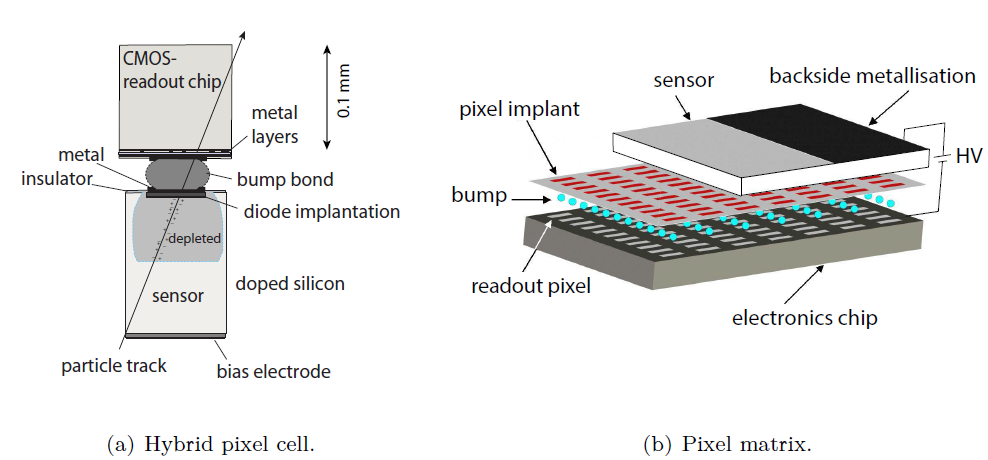
\includegraphics[scale=.6]{hybrid}
\caption{On the left (a), the structure of a single pixel cell, made by the sensor and the electronic readout. On the right (b), an exploiting representation of the entire hybrid pixel matrix arrangement.}
\label{fig:hybrid}
\end{figure}

In a few words, when a particle crosses the sensor, a signal is generated on the electrodes due to the drift of the charge carriers in the depleted region. This signal passes through the conductive bump in the readout chip, where it is amplified and discriminated.

Oen of the advantage of the pixel detectors with respect to the strip sensors, is the higher tolerance to radiation damage. The \emph{leakage current} increses as the radiation doses become higher, and it depends on the volume of the sensors and it is distributed over all electrode. Thus, in pixel detectors this current is shared among more electrodes with respect to the strip detectors. So the leakage current per electrode is smaller. Moreover, as separate entities, sensor and readout coul be independently optimize.
Among the disadvantages instead, there are the cost and complexity of the implementation processes, but also large material thickness together with the necessity to add support and cooling structures, which worsen the track reconstruction and momentum resolution because of the multiple scattering.
%LEAKAGE
[NOTE ON LEAKAGE]

\subsection{Monolithic pixel detector}

We have seen that hybrid detector are made by two separate structures: the active sensor and the passive readout chip, connected by micro-connections. Since both of them are made of silicon, in principle, it could be possible to build them in a monolithic unit. In this way the amount of material decreases, enhancing the tracking performance and momentum resolution. 

Developments of this sensors have tried to exploit industrially already available technologies, like CMOS technologies. They have to reach a large depletion zone in order to improve the signal-to-noise ratio, but also design electrode with small capacitance, to reduce the noise. High radiation tolerance is also required.
[note on capacitance, influenza power consumption]
%CAPACITANCE???

An example of this type of sensor is the DEPFET pixel detector, which contains only one active transistor in every pixel pixel. Monolithic Active Pixel Sensors (MAPS) employed CMOS technologies to include a readout circuit in their structure and we will see them in more details in~\autoref{sec:MAPS}

\begin{description}
\item[Depleted p-channel field effect transistor (DEPFET)]
\end{description}

In a DEPFET pixel detector, each pixel implements only one transistor. In~\autoref{fig:DEPFET} is shown an example of a DEPFET pixel.

\begin{figure}[h!]
\centering
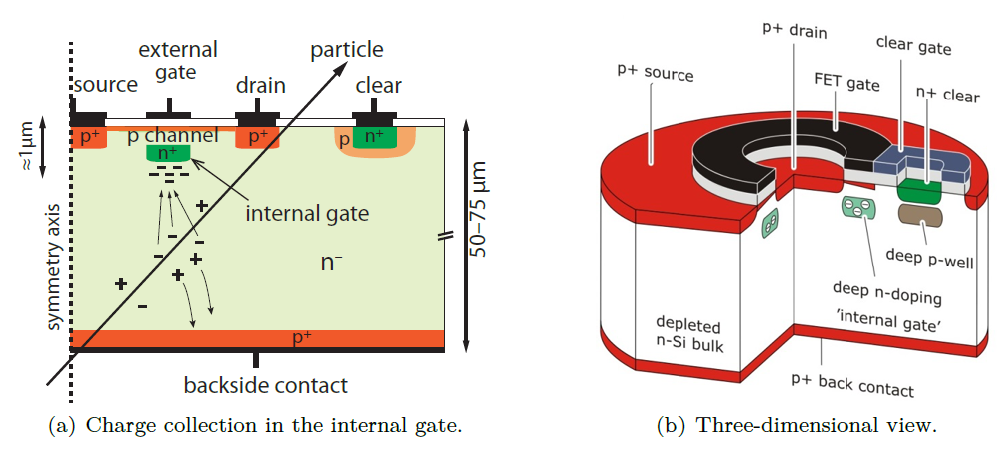
\includegraphics[scale=.6]{DEPFET}
\caption{On the left (a) a cross section of a circular DEPFET pixel cell, where the charge collection is also sketched. On the right (b), a three-dimensional view of the same pixel cell.}
\label{fig:DEPFET}
\end{figure}

The depletion region extends between the backside $p^{+}$ contact and the several $p^{+}$ regions near the transistor element (drain, source and a $n^{+}$ clear contact installed in a p region) and the $n^{-}$ substrate. When a traversing particle releases energy, ionizing the medium, electorns drift towards the top surface, and the holes towards the backside due to the external potential.\\
The transistor is a p-channel MOSFET that produces a hol current from source to drain, controlled by the potential on the external gate. Moreover, there is als a deep $n^{+}$ implant placed under the transistor, a few micrometers away. It is the most positive point in the pixel structure and so it is a local minimum for the electrons. In fact this implant features an electron accumulation, which changes the potential making it an \textit{internal gate}. 
Electrons collected on this electrode, influences with the external gate the current flow in the DEPFET transistor channel. After the measurement, they are removed applying a positive voltage on the \textit{clear contact}. In order to not compete as a collection electrode for the electrons, this element in embedded in a p region (\textit{deep p-well}).\\
With some variations in the pixel structure, this is the type of sensors that PXD is made of.

\section{CMOS Monolithic Active Pixel Sensors technology} \label{sec:MAPS}
 
First prototypes of pixel detector, which employed the CMOS technology to fabricate both the sensor and the readout circuit in the same silicon die, date back to the early 1990s. FUrther developments have led to the \emph{monolithic active pixel sensors} (MAPS) with an epitaxial[NOTE?] silicon layer for charge collection (at most diffusion?) and then to the Depleted MAPS (DMAPS), where the depleted region is extended throughout the volume. CMOS is the essential feature that have allowed to realize this delicate and complex detectors.

\subsection{MAPS pixel detectors}

This type pf sensors have been exploited the CMOS tehnologies for optical application, where the structure have an epi-layer with high resistivity to detect the light, and the electronic circuitry on the top of it. In this case, not the entire area is sensitive to the charge production. The effectively active fraction of the pixel area is called \textbf{fill factor}. 
In~\autoref{fig:MAPS_fig} is shown a schematic of their structure. 

\begin{figure}[h!]
\centering
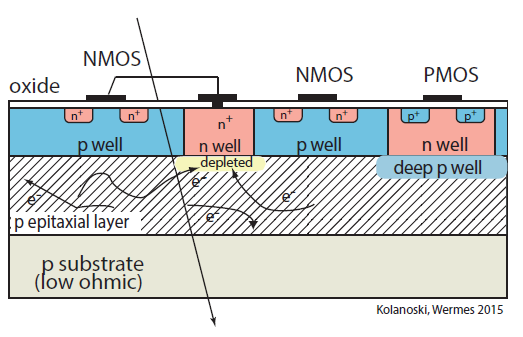
\includegraphics[scale=.7]{MAPS}
\caption{Schematic of a monolithic pixel detector (MAPS).}
\label{fig:MAPS_fig}
\end{figure}

In MAPS pixel detector, charge collection is mostly achieved by diffusion, because the sensitive region is not fully depleted. The collection electrode is a $n^{+}$ contact in a n-well, embedded in a p-epitaxial layer (highly resistive?) put on the top of a p substrate (low ohmic). Other n-wells can be necessary, for example to host PMOS transistors, and for this reason they have to be shielded by deep p-well, to prevent them to become competitive for charge collection. These highly doped deep layers assume a negative potential with respect to the collection electrode and hence a repulsive effect.
Due to the absence of a drift field in theepi-layer, with the exception of the region immediately below the collection electrode, collection charge occurs mainly by diffusion and thus it is slow and incomplete. 
Typical values of the epi-layer thickness are within the range of 1 - 20 $\mu$m.

Maps detector can't be used in high rates experiments because they have charge collection time of the order of 100 ns, thus too slow and also a not very suitable radiatin tolerance.  But they have successfully employed for heavy ions collisions, like STAR experiment at RHIC (Relativistic Heavy Ion Collider) and the ALICE upgrade at the LHC[chip pALPIDE articolo 1]. [In fact they do not require complex bump-bonding processes and they could be produced in large volumes, so they result ideal for large dimension experiments.]

%DIMENSIONI TIPICHE

\subsection{Depleted MAPS pixel detectors}

In order to obtain fast and fully collection of released charge, it is necessary to drift the carriers toward the electrodes, by an external elective field. A fully depletion of the sensitive zone, enhance the charge collection, producing large signal (and thus a better signal-to-noise ratio). \\
The depletion depth depends on the substrate resistivity and the bias voltage, according to the relation:

\begin{equation}
d \propto \sqrt{\rho V}
\end{equation}

For this reason, new processing techniques have been employed to allow applying higher voltage or process high-ohmic substrate wafers. Both of them are used to increase the depletion region and so to provide large and fast signal.
%HOGH RESISTIVITY SUBSTRATE

We can distinguish two main variants of DMAPS pixel detector: with a \textit{large} or \textit{small} collection electrode, shown in~\autoref{fig:fill_factor}.

\begin{figure}[h!]
\centering
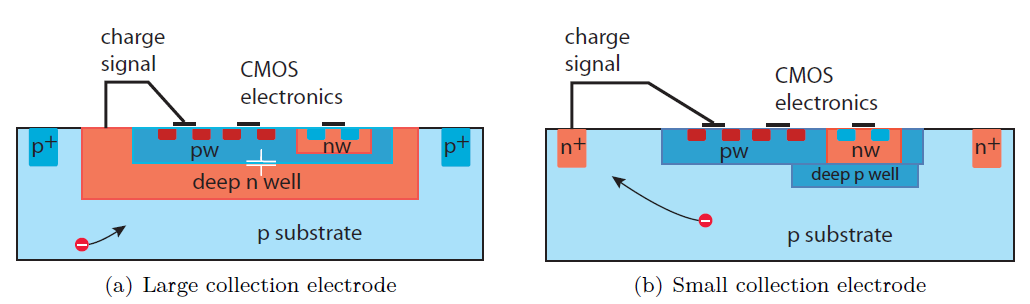
\includegraphics[scale=.6]{fill_factor}
\caption{On the left (a) a schematic of the large electrode design. On the right (b) the small electrode design.}
\label{fig:fill_factor}
\end{figure}

The \textit{large collection electrode} DMPAS features a deep n-well which acting as electrode but also as shield for the entire CMOS electronics for the readout, which is embedded within it. This architecture improve the radiation tolerance because the reduced average drift distance of the charge carriers decreases the probability of trapping. At the same time though, large size of the electrode implicates higher values of capacitance (several hundred fF) which increases the noise and worsens the timing performance.\\
The \textit{small collection electrode} variants has a small n-well collection node, distanced from the CMOS circuitry which is embedded in p-well and deep p-well layers (following the logic of the opposite doping?). In this design, low capacitance of about 5-20 fF can be obtained, improving noise and timing performance.
Radiation tolerance instead, is more difficult to reach due to larger average distance travelled by the carriers. Smaller pixel dimensions are preferred for small electrode (to reduce the path), and therefore higher power density is accepted in exchange of increased robustness against radiation.\\

%TRAPPING 
[NOTE ON TRAPPING]

%DIMENSIOINI TIPICHE

However a additional modification of the technology have allowed to further improve radiation tolerance. In~\autoref{fig:n_doped} is displayed an example.\\

\begin{figure}[h!]
\centering
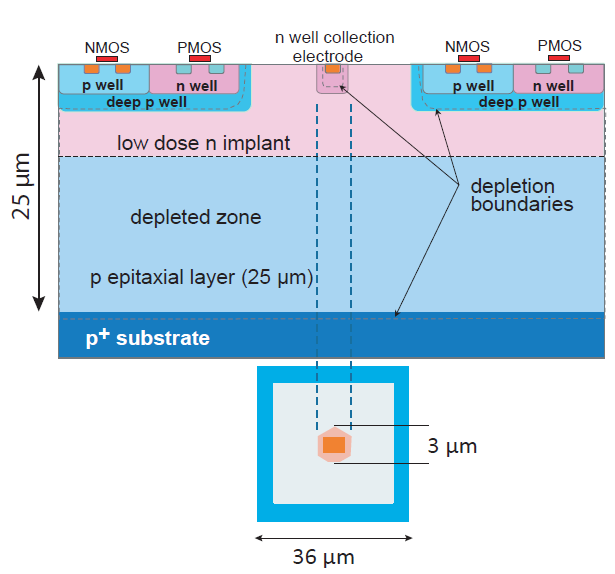
\includegraphics[scale=.7]{n_doped}
\caption{Small electrode design with the addition of a low n-doped layer.}
\label{fig:n_doped}
\end{figure}
%CONTROLLA CAPTION

The epi-layer is depleted from two pn junctions: the deep p-wells and the low dose n-implant, the n-implant and the p-epitaxial layer[CITE ARTICOLO 2]. This addition creates a potential minimum for electron collection underneath the deep p-well with a field direction towards the n collection well, thus strengthening collection of charges laterally[CITE]. The epi-layer is 25 $\mu$m thick and the collection electrode is on positive potential. [ESEMPIO DI SEGNALE CON CAPACITAE CARICA RILASCIATA.]
%IMMAGINE CAMPO ELETTRICO? NO SENSOR CAPACITANCE PENALTY


\subsection{Silicon On Insulator (SOI) technology}

\textit{Silicon on Insulator} (SOI) technology represents another way to combine the sensitive region and the readout circuit in a single monolithic unit. In this architecture, the transistor is isolated by vertical trenches and is divided from the bulk by a $SiO_{2}$ layer, called \emph{buried oxide} (BOX).
An high resistivity bulk wafer allows to depleted the volum in the region below the BOX, in order to generate a large charge signal when a particle pass through the detector. The bulk and the CMOS electronics are connected by vertical connections, called \textit{vias}. \\
In~\autoref{fig:SOI_fig} is displayed a monolithic SOI pixel, with a doped volume placed between the CMOS circuitry and the BOX. This variation prevents the capacitive coupling from the substrate into the electronics, through the BOX.

\begin{figure}[h!]
\centering
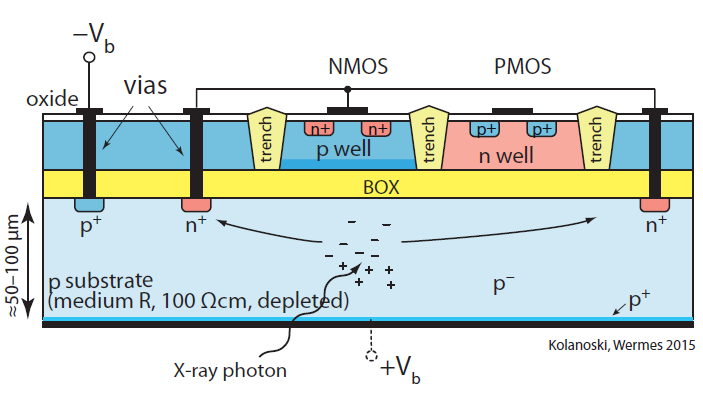
\includegraphics[scale=.7]{SOI_fig}
\caption{An example of a Monolithic SOI pixel.}
\label{fig:SOI_fig}
\end{figure}


\section{History of Monopix developments}

As we have try to show in the previous, in recent years, advances in CMOS technologies have led to the development of a new generation of monolithic pixel sensors (DMAPS) with fast readout and high radiation tolerance. For this reason these new devices become promising candidate for high-energy physics experiment with high rate and high radiation environment.


\subsection{Developments of DMAP devices}

Specifically two different lines of DMAPS development have been followed, distinguished by different pixel architectures, entrusted to two different implementation process technologies:

%charge sensitive amplifier in large and voltage in small??
\begin{itemize}
\item \textbf{large fill factor} line: with large collection electrode and the electronics inside the charge collection well, these prototypes are indicate to experiments with high rate and high radiation conditions, because they could ensure a greater tolerance to huge doses of radiation. They have been fabricated in LFOUNDRY 150 nm design. [REFERENCE] In~\autoref{fig:LF} are shown some of these chip development.
\item \textbf{small fill factor} line: small collection electrode and the electronics outside the charge collection well, these devices need a process modification to enhance the radiation hardness, but they are faster and due to less values of total capacitance, they implicate much less power consumption, with respect to the previous. These devices instead, are fabricated ina modified() TowerJazz 180 nm CMOS imaging process.
\end{itemize}

\begin{figure}[h!]
\centering
\subfigure[CCPD\_LF]
{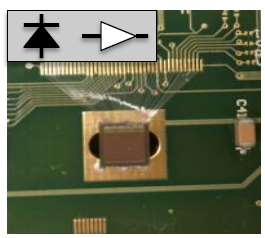
\includegraphics[scale=0.6]{LF1}}\quad
\subfigure[LF-CPIX]
{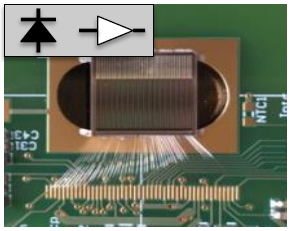
\includegraphics[scale=0.6]{LF2}}\quad
\subfigure[LF-MONOPIX 1]
{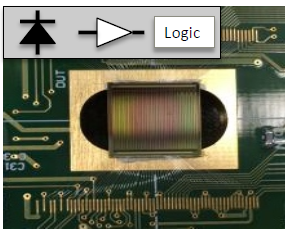
\includegraphics[scale=0.6]{LF3}}\\
\caption{LFOUNDRY 150 nm development line.}
\label{fig:LF}
\end{figure}

%immagine wermes talk

\subsection{TJ-Monopix line}

In~\autoref{fig:TJ} are displayed the major prototypes that have allowed to design the last iteration of this series, TJ-Monopix 2, whose characterization results will be shown in~\autoref{ch:TJ2}.

\begin{figure}[h!]
\centering
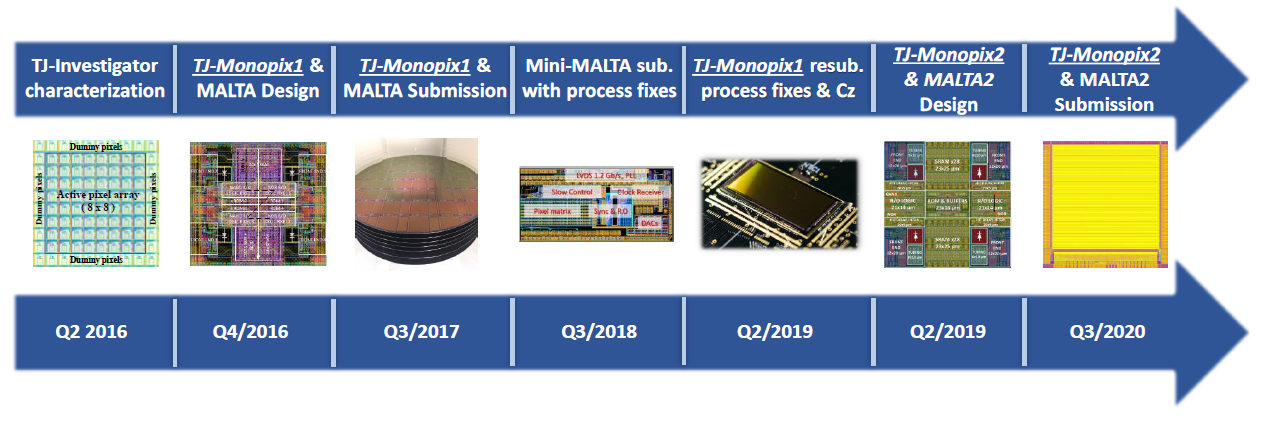
\includegraphics[scale=.55]{TJ}
\caption{TowerJazz 180 nm development line.}
\label{fig:TJ}
\end{figure}

The standard TJ 180 nm process has been employed to realize the ALPIDE (sigla) monolithic active pixel sensor, selected for the ALICE Inner Tracking System (ITS) upgrade [reference].
The chip proved to be suitable for the modest ALICE requirements, but the standard process do not ensure the full depletion volume, which is crucial to limit the signal degradation expecially after irradiation. For this reason, the aforementioned process modification have been developed by CERN in collaboration with the foundry [cite and reference], that allows full depletion of sensitive layer. This new implementation has been tested in a dedicated chip called TJ-Investigator, and the obtained results have been demonstrated the effectiveness of the modified process. \\
Therefore two large scale demonstrator chips have been realized, called TJ-Monopix1 and TJ-Malta1, whose main difference lies in the different readout architecture. The TJ-Malta1 chip implemented an \textit{asynchronous} readout architecture, which eliminate the Bunc Crossing ID (BCID, timestamp), in order to reduce the digital power consumption. For TJ-Monopix1 instead, a \textit{coulmn-drain} readout architecture was chosen, which will be described in the following. Both chips have been fully tested and irradiated to investigate their functionality and efficiency, which however has decreased from 97 \% to 70 \% after irradiation. The reason was address to the weak lateral field at the pixel edge, so the process has been further optimized in order to resolve this issue and another chip, called mini-Malta, was implemented with this variation to test its efficiency. Results show significant improvement, thus it was implemented in the original Tj-Monopix1 and TJ-Malta1 chips.
The variation consist in two different structure of the pixel, displayed in~\autoref{fig:enhance_lat} called \textbf{Full deep p-well (FDPW)} and \textbf{Removed deep p-well (RDPW)}. As we can see, the deep p-well underneath the CMOS electronics is reduced at the pixel edge in case of RDPW structure. It can be seen the significant improvement of the electric lateral field, which results in turn in faster charge collection and so high efficiency even after irradiation.
%[REFERENZE VARIE]

\begin{figure}[h!]
\centering
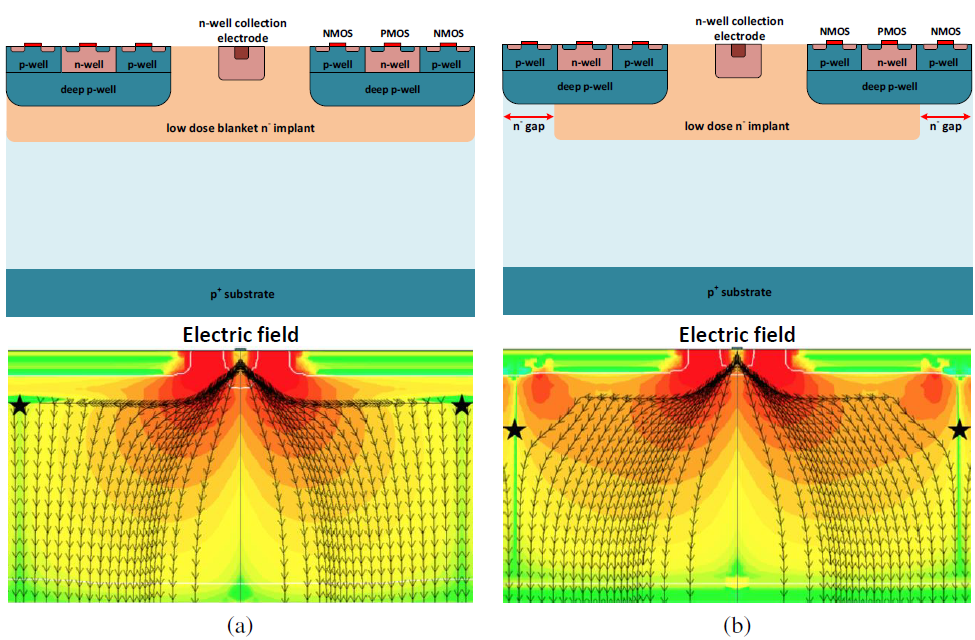
\includegraphics[scale=.7]{enhance_lateral}
\caption{In the left, the Full deep p-well (FDPW) structure and its lateral electric field, compared with te Removed deep p-well (RDPW) variation. Both of them implemented the process modification with a low dose n implant.}
\label{fig:enhance_lat}
\end{figure}

%RIVEDI EXTRA DEEP P WELL

Further optimization of the pixel size, which is critical to take full advantage of field shaping through process modifications and to improve charge collection, have been implemented in the last iteration of this development line: TJ-Monopix2, considered as starting point for the development of the OBELIX final chip, designed for the upgrade of the Belle II vertex detector.  

%FDPM RDPW as further modification and imrpvement of lateral field???[reference]

Now we want to describe the readout architecture chosen for TJ-Monopix2, which will crucial in the following. 

\begin{description}
\item[The Column-drain readout architecture(pag.42)]
\end{description}

The \textit{column-drain} architecture implemented in TJ-Monopix ensures fast readout by encoding the analog charge information using the standard \textbf{Time Over Threshold (ToT)} technique. This procedure exploits two timing information: the \textbf{Leading Edge (LE)} which correspond to the hit time of arrival (when the signal valueS goes beyond the threshold), and the \textbf{Trailing Edge (TE)} that is when the signal goes below the threshold value. From the difference between the TE and the LE, the ToT can be calculated. 
The \textit{in-pixel} circuitry implemented a Random Memory Acces (RAM) where to store the LE and TE timing info, a Read-Only Memory to store the pixel address and the control and arbitration logic, which we will see more about in the following. 
The readout is \textit{column-based}, so all pixels of each double column share a common column-bus which could be accessed by one pixel at a time, with a defined priority logic. The column bus includes the BCID timestamp, the data (LE, TE, address) and the control signals.
The \textit{periphery} includes the End Of Column (EoC) block which deals with the transmission and readout of the column-bus signals, and the Digital Chip Bottom (DCB), that instead, processes the hit information. 
The readout could be triggere or full-readout. In TJ-Monopix line follow the second type, hit data is continuously transmitted to the DAQ. In case of triggered readout, hit data is stored in a trigger memory, and the information is transmitted only when the trigger signal arrives.

\begin{figure}[h!]
\centering
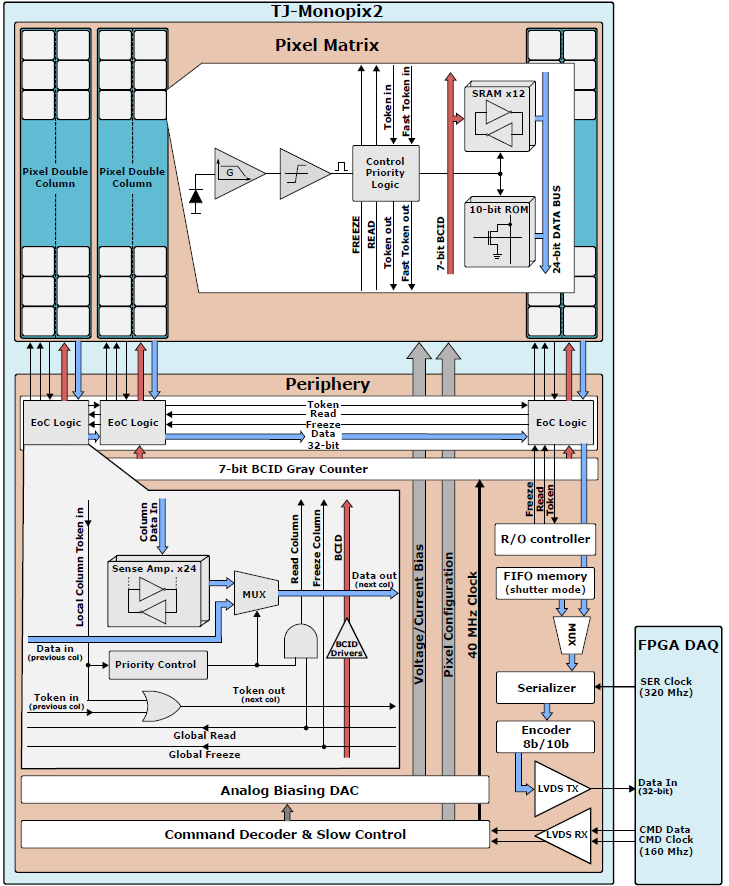
\includegraphics[scale=1]{RO}
\caption{Architecture of TJ-Monopix 2.}
\label{fig:RO}
\end{figure}

In~\autoref{fig:RO2} is displayed an example of the readout of two hits. The readout sequence starts when the TEcpulse arrived. A hit flag is set and it acivates the \textsc{\textbf{TOKEN}} signal, which in turn is arised to warn that the pixel is available to be read out. This signal propgates across the double column with a priority logic until it arrives to a readout controller, which uses other two global signals, the \textsc{\textbf{FREEZE}} and \textsc{\textbf{READ}}, to control the readout progression. They are distributed to across the EoC blocks and local copies are transimitted only to the double column that has been hit and that has the higher priority (It is a different priority logic among each double column which goes from left to right across the matrix).
The first ensures that new hits do not interrupt the pixel priority logic setting other new hit flag, which means that they could not transmit new hit information. In this way the pixel priority in the readout sequence is well defined. The latter instead, allows to the pixel with the hit flag and highest priority to access the data bus and transmit the hit information to the periphery. A series of \textsc{\textbf{READ}} cycles allow all pixel in the sequence to be read out.

\begin{figure}[h!]
\centering
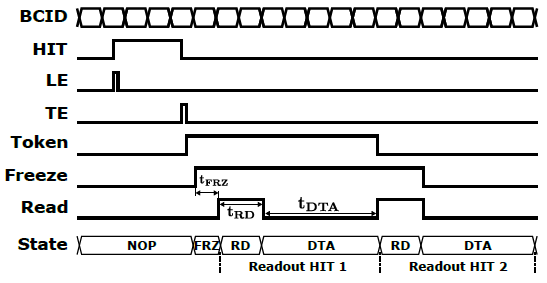
\includegraphics[scale=.9]{RO2}
\caption{?}
\label{fig:RO2}
\end{figure}

%pag 164 tesi, addition of 8-bit column address by EoC

%ToT (thesis immagine pag 31, 34)\\






% ARTICOLO 0 (INIZIO TESI)
%CAPITOLO 8 
% MUSTAKAS THESIS
% ARTICOLI VARI
% PRESENTAZIONI






















































%-----------------------------------------------------------------------------------------------

%COMMENT



% PRIMA IPOTESI INTRODUZIONE -> SPIEGARE BETHE-BLOCH
\begin{comment}
The detection of elementary particles, nuclei and radiations occurs through their interactions with matter. For example, charge particles are detected by ionization of matter along the trajectory o through the emission of electromagnetic radiation (bremsstrahlung, Cherenkov and transition radiation). Electrons and photons usually develop \textit{electromagnetic showers} in matter. So, all of them interacts by \emph{electromagnetic force}.
Neutrons and other hadrons instead, are revealed employing the \emph{strong interaction} through the formation od \textit{hadronic showers}. Neutrinos, eventually, are detected exploiting the \emph{weak interaction}.

Here we want to sift though the main aspects which characterize the detection of charged particles. 

\subsection{Energy loss by ionization}

The dominant processes which affect the energy loss of charged particles in matter is ionization and excitation of the medium's atoms, at least until the particles reach such high energy that they begin to lose it through radiation.

The average energy loss results from a series of individual stochasti processes, and its behaviour per path lenght is described by the \textit{Bethe-Bloch formula}:

\begin{equation}
-\biggl\langle \frac{dE}{dx} \biggr\rangle = K \frac{Z}{A} \rho \frac{z^{2}}{\beta^{2}} \biggl[ \frac{1}{2} \ln(\frac{2m_{e}c^{2}\beta^{2}\gamma^{2} T_{max}}{I^2}) - \beta^{2} - \frac{\delta(\beta\gamma)}{2} - \frac{C(\beta\gamma,I)}{Z} \biggr]
\label{eq:bethe}
\end{equation}

All the various quantities are explained above:

\begin{itemize}
\item $K = 4\pi N_{A} r^{2} m_{e} c^{2}$ = 0.307 MeV $cm^{2} mol^{-1}$, with the elctron radius $r_{e} = \frac{e^{2}}{4\pi \epsilon_{0} m_{e} c^{2}} \approx 2.8 fm $
\item Z, A, $\rho$ are the atomic number, the atomic mass and the density of the medium, respectively.
\item $z, \beta$ are the charge and the velocity of the particle passing through the matter.
\item I is the mean excitation energy, which describes how easily a target, typically a molecule or atom can absorb kinetic energy from the projectile.
\item $T_{max}$ is the maximum energy that is possible to transfer to a shell electron in a central collision.
\item $\delta$ is the \textit{density correction}, which takes into account a relativistic effect that is the increasing transverse extension of the electric field with $\gamma$.
\item $\frac{C}{Z}$ is a shell correction, relevant for small $\beta$ values.
\end{itemize}

[description of the curve?]

The Bethe-Bloch formula describes the mean energy loss of particles traversing a medium and so it is also called \textit{\textbf{stopping power}}. 
As we mentioned above, the energy loss process has a statistical nature, because it is determined by many ionization or excitation cases, which contributes individually to the formula. Both the number N of total processes and the emitted energy in each one of them, produce fluctuation in the enrgy lost by a particle and as consequence of the energy deposited in the material. They are known as \textit{Landau fluctuations} and they can influence the performance of detectors, so they must be considered. For example in particle identification by the measurement of $\< dE/dx \>$, these fluctuations widen the width of the distribution, worsening the resolution in distinguishing different particle species. In tracking detectors instead, they reduce the space resolution.

[bremss]

\end{comment}


\begin{comment}
There are two type of motions affecting charge carriers moving in electric and magnetic field:

\begin{itemize}
\item An unordered motion with a velocity distribution, classically decribed by the Maxwell-Boltzmann distribution, valid in thermal equilibrium and in absence of an electric field. For example, if there is a concentration gradient in the medium, charges created locally tend to diffuse causing a dispersion of the local charge distribution.
\item A drift movement determined (induced) by the presence of the external electric and magnetic fields. The \textit{drift velocity} $\vec v_{D}$ is the result from a balance between the electric force that aceelerates the charged particles and a friction force arising from collisions with atoms and molecules. In most cases drift velocity is much smaller then the mean velocity $\bigl\langle v \bigr\rangle$.
\end{itemize}

The charge carriers motion in semiconductors is described by the Boltmann transport equation () which includes both diffusion and drift motions (figure). However a specific account on the motion of charge carriers is necessary because lattice phenomena have to be taken into account. 

\begin{description}
\item[DRIFT MOTION]
\end{description}

\begin{description}
\item[DIFFUSION MOTION]
\end{description}

\end{comment}




